\section{Abast}{0}
L'objectiu del projecte \'{e}s desenvolupar un conjunts de serveis web per manegar l'algoritme de identificaci\'{o} de fonts bacteriol\`{o}giques Ichnaea. Actualment Ichnaea es troba en la versi\'{o} 2.0, desenvolupat per Aitor P\'{e}rez P\'{e}rez. La primera versi\'{o} va ser desenvolupada per David Sanchez.\\

La complexitat de les dades i configuracions dels parametres de entrada de Ichnaea, requereixen d'unes interf\'{i}cies i d'un model de dades flexible per poder executar l'algoritme de forma m\'{e}s amigable i comprensible. El prop\`{o}sit del projecte es dissenyar e implementar aquest sistema en un entorn distribu\�{i}t en xarxa.\\

En col.laboraci\'{o} amb Miguel Ibero, que desenvolupa com a Projecte de Final de Carrera un sistema de cues per manegar les execucions de Ichnaea, integrarem una primera versi\'{o}.\\


\section{L'univers Ichnaea}{1}
Per tal de poder entendre els objectius del projecte farem una visi\'{o} global de Ichnaea i els seus elements.\\

\subsection{MST: Microbial Source Tracking}
MST \'{e}s un problema obert en l'actualitat. Consisteix en determinar l'origen biol\`{o}gic dels residus fecals en cossos aquosos mitjan\c{c}ant l'\'{u}s d'indicadors qu\'{i}mics i microbiol\`{o}gics \cite{paper}. Per fer aix\'{o} es prenen mostres i s'analitzen en un laboratori, i segons els resultats, es decideix si contenen residus fecals d'origen hum\`{a} o de quina familia de animals \cite{pfc}.\\

Pendre aquesta decisi\'{o} \'{e}s molt dif\'{i}cil. Fins i tot, els microbi\`{o}legs no estan completament segurs de determinar la font d'infecci\'{o} de les mostres d'aigues contaminades. La ra\'{o} \'e{s} que les mostres son extretes directament de l'entorn i per aix\'{o} estan diluides i envellides \cite{pfc}.\\

L'estudi de l'origen de la pol.luci\'{o} en cossos aquasos \'{e}s un problema gran i pot ajudar a assegurar la protecci\'{o} de les poblacions humanes, mostrant una varietat d'enfermetats, especialment en paisos subdesenvolupats \cite{pfc}.\\

\subsection{Ichnaea 2.0}
Ichnaea \'{e}s un software desenvolupat per ajudar a resoldre el problema MST. \'{E}s un eina per llegir matrius de dades(mostres mesurades) i ensamblar diversos conjunts de models. Amb l'ajuda d'aquestes bosses de models, pot llegir noves mostres i fer prediccions dels origens d'aquestes \cite{pfc}.\\

Desde la primera versi\'{o} s'ha refactoritzat el codi i millorat tant el rendiment com els algoritmes.\\

\section{Objectius}
\subsection{Visi\'{o}}
Aquest projecte consisteix en desenvolupar un sistema web dissenyat per executar Ichnaea. Desde el principi ofereix  m\'{e}s funcionalitats que les que dona de base Ichnaea 2.0. L'objectiu \'{e}s poder aprofitar aquest sistema per les futures versions de Ichnaea. Degut a que la execuci\'{o} \'{e}s complexa i de temps elevat, existeix una part del sistema desenvolupada per Miguel Ibero, amb qui es col.labora activament. Aquesta part \'{e}s un sistema de cues per administrar les execucions del software.\\

\subsection{Objectius assolits}
\begin{itemize}
\item Estudi de tecnologies per la implementaci\'{o}. El per\'{i}ode de investigaci\'{o} ja s'ha portat a terme. Finalment s'est\`{a} implementant amb un framework de codi lliure Symfony2 \cite{symfony} amb Data Mapper Doctrine \cite{doctrine} per a MySQL \cite{mysql} i motor de templating TWIG \cite{twig}. Totes han sigut tecnologies que s'han apr\'{e}s desde 0.

\item Sistema web. Implementar tots aquests objectius en una tecnologia distribuida en xarxa. S'ha aplicat desde el principi tecnologia web usant Symfony2 Framework \cite{symfony}.

\item Model de dades. Dissenyar un model de dades flexible que permiti relacionar els objectes per a futures versions de Ichnaea i noves funcionalitats que es poguin desenvolupar mitjan\c{c}ant modificacions o millores de les interf\'{i}cies. S'est\`{a} dissenyant de base un model de dades flexible amb un motor de base de dades relacional. Per\'{o} actualment s'est\`{a} limitant la flexibilitat a nivell de interf\'{i}cie per obtenir una millor experi\`{e}ncia d'usuari.

\item Interf\'{i}cies d'entrada del sistema. Especificar e implementar les interf\'{i}cies d'usuari per poder configurar les entrades i execuci\'{o} del software Ichnaea. S'han especificat e implementat quasi totes les interf\'{i}cies de entrada. 

\item Interf\'{i}cies de sortida del sistema. Especificar e implementar interficies de usuari per poder veure els resultats de la execuci\'{o} del software Ichnaea. S'han especificat e implementat quasi totes les interf\'{i}cies de sortida. 

\item Disseny de interf\'{i}cies complexes. Interf\'{i}cies usables, comprensibles i enriquides per tenir una bona experi\`{e}ncia d'usuari. La configuraci\'{o} de les matrius \'{e}s la m\'{e}s complexe. S'ha acomplert aquest objectiu mitjan\c{c}ant una API JSON Restful \cite{apijson} amb les interf\'{i}cies enriquides amb Javascript i Jquery\cite{jquery}, juntament amb una proto-llibreria pr\`{o}pia pel software.

\item JSON Api RESTful \cite{apijson}. Prototipus de llibreria API per en un futur escalar-la i poder integrar el projecte amb qualsevol perif\`{e}ric o tecnologia. Objectiu assolit ja que era requeriment de l'objectiu anterior. Aquesta API es probable que creixi en funcionalitats.

\item Dissenyar un sistema i emprar unes tecnologies escalables i mantenibles. El projecte \'{e}s un prototipus i ofereix m\'{e}s funcionalitat que les que oficialment ofereix Ichnaea. A mesura que Ichnaea ofereixi m\'{e}s funcionalitats, el sistema web est\`{a} dissennyat per que sigui mantenible en el futur amb documentacions per a desenvolupadors acurades. El fet d'usar Symfony2 \cite{symfony} ens assegura una bona qualitat de documentaci\'{o} generada per la comunitat i actualment \'{e}s un dels frameworks m\'{e}s reconegut a nivell mundial.

\end{itemize}

\subsection{Objectius per assolir}
\begin{itemize}
\item Interf\'{i}cies d'entrada de prediccions. Falten especificar e implementar les interf\'{i}cies de les entrades predicci\'{o}.
\item Interf\'{i}cies de sortida de prediccions. Falten especificar e implementar les interf\'{i}cies de les sortides de predicci\'{o}.
\item Demostracions i modificacions. Es far\`{a} una demostraci\'{o} al client final i s'establiran dos per\'{i}odes de modificacions.
\item Integraci\'{o} amb cues. Integrar la aplicaci\'{o} web amb el projecte ''Sistemes de cues per Ichnaea Software'' de Miguel Ibero. Aquesta integraci\'{o} t\'{e} dues parts: entrenaments i prediccions. El projecte est\`{a} integrat amb la primera part per\`{o} encara es troba en desenvolupament la segona part. 
\item Prototipus en un entorn producci\'{o}. Actualment el desenvolupament es troba actualitzat al RdLab. Cada dos setmanas es puja la ultima versi\'{o}. Es col.labora amb Miguel Ibero per poder donar una entorn de explotaci\'{o}.
\item Manuals. Manual d'usuari, d'administrador, de desenvolupadors i de administradors de sistema.
\end{itemize}

\section{Planificaci\'{o}}
La planificaci\'{o} per la realitzaci\'{o} de les taquest per assolir \'{e}s la seg\�{u}ent, on cada columna representa una setmana.
\begin{figure}[h!]
  \centering
  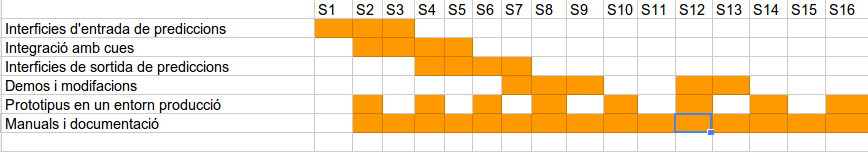
\includegraphics[scale=0.5]{gant.png}
  \caption{Planificaci\'{o}}
  \label{fig:placement}
\end{figure}

\begin{thebibliography}{9}
\bibitem{pfc}Aitor P\'{e}rez P\'{e}rez ''ICHNAEA 2.0: a software for microbiology modelling'' pp. 7-34, Feb. 2014

\bibitem{paper}D. S\'{a}nchez ''A Software System for the Microbial Source Tracking Problem'' 2012

\bibitem{symfony} ''Learn Symfony - Symfony'' [Online]. Disponible a ''http://symfony.com/com/doc/current/index.html

\bibitem{apijson} ''JSON API''  [Online]. Disponible a ''http://jsonapi.org''

\bibitem{jquery} ''jQuery: The Write Less, Do More, JavaScript Library'' [Online]. Disponible a ''http://jquery.com''

\bibitem{doctrine} ''The Doctrine Project'' [Online] Disponible a ''http://www.doctrine-project.org''

\bibitem{mysql} ''MySQL :: The world's most popular open source database'' [Online] Disponible a ''http://www.mysql.com''

\bibitem{twig} ''Twig - The flexible, fast, and secure PHP template engine''  [Online] Disponible a ''http://twig.sensiolabs.com''
\end{thebibliography}
